\documentclass[9pt]{beamer}


\usepackage{adjustbox}
\usepackage{algorithm}
\usepackage{algpseudocode}
\usepackage{amsfonts}
\usepackage{amsmath}
\usepackage{amssymb}
\usepackage{amsthm}
\usepackage{array}
\usepackage{blindtext}
\usepackage{cite}
\usepackage{cuted}
\usepackage{caption}
\usepackage{environ}
\usepackage{graphicx}
\usepackage{grffile}
\usepackage{hyperref}
\usepackage{import}
\usepackage{lmodern}
\usepackage{mathtools}
\usepackage{microtype}
\usepackage{multirow}
\usepackage{pgfgantt}
\usepackage{pgfplots}
\usepackage{physics}
\usepackage{setspace}
\usepackage{siunitx}
\usepackage{stfloats}
\usepackage{subcaption}
\usepackage{tikz}
\usepackage{url}
\usepackage{xcolor}
\usepackage[acronym]{glossaries-extra}
\usepackage[font=footnotesize,labelfont=bf]{caption}
\usepackage[RPvoltages]{circuitikz}
\usepackage[T1]{fontenc}
\usepackage[short]{optidef}

% tikz/pgf
\pgfplotsset{compat=newest}
\usetikzlibrary{plotmarks}
\usetikzlibrary{arrows.meta}
\usepgfplotslibrary{patchplots}

% amsthm
\newtheorem{proposition}{Proposition}

% siunitx
\DeclareSIUnit{\belmilliwatt}{Bm}
\DeclareSIUnit{\dBm}{\deci\belmilliwatt}

% blindtext
% \newcommand\blfootnote[1]{%
% \begingroup
% \renewcommand\thefootnote{}\footnote{#1}%
% \addtocounter{footnote}{-1}%
% \endgroup
% }

% caption
\captionsetup[figure]{labelformat=empty}

% glossaries-extra
\setabbreviationstyle[acronym]{long-short}
\newacronym{af}{AF}{Amplify-and-Forward}

% \setlength{\abovedisplayskip}{0pt}
% \setlength{\belowdisplayskip}{0pt}
% \setlength{\abovedisplayshortskip}{0pt}
% \setlength{\belowdisplayshortskip}{0pt}

\usetheme{Warsaw}
\title[Semantic Communications: An Introduction]{\LARGE{\textbf{Semantic Communications: An Introduction}}}
\subtitle{Group Presentation}
\author{Yang Zhao}
\institute{Department of Electrical and Electronic Engineering\\Imperial College London}
\date{\today}

% ! communications from engineering perspective (Shannon) and everyday perspective
% ! transmitter and receiver becomes higher level (task- or human-oriented), with conventional transmitter and receiver as subsystem
% ! error may due to losses in any source coding, noise in the channel, or their combinations.
% ! different background knowledge or inference rules, memories, feedbacks
% ! the presence of background knowledge reduces the informativeness of the source; However, if the background knowledge is shared, the reduction in semantic entropy means that we can compress the source without losing information: source information is the same amount, but can be compressed based on receiver's knowledge
% ! in Shannon’s theory, the information of a message is governed by its __statistical probability__ but not its meaning (e.g., whether the message itself is true or false).
% ! in Carnap and Bar-Hillel’s formulation, the statistical probability p(s) is irrelevant, and the semantic information of s is determined by its __logical probability__ P p(w) under w|=s their language system.
% ? transmitter and receiver should 1) have some shared (e.g., file type) and local knowledge (e.g., purpose), which can be ``of higher level''; 2) the message generator has great freedom in picking a ``good'' code: accurate, easy to generate, destination interested in (redundancy and reliability).
% * example on CSIT (channel state information at the transmitter; classical semantic information theory)
% ! semantic world: every thing (message) is absolutely true or false
% ? background can be memory- or learning-based results, some semantic communication is enabled even if no physical channel
% ! there is still a gap between visual features and semantics
% * example on dog classification: why not classify at tx and transmit result only? local knowledge, how much content to transmit for just right decision?
\begin{document}

\begin{frame}
	\titlepage
\end{frame}

\begin{frame}{Table of Contents}
	\tableofcontents
\end{frame}

\begin{section}{Theory}
	\begin{frame}{Shannon's Information Theory}
		\begin{figure}
			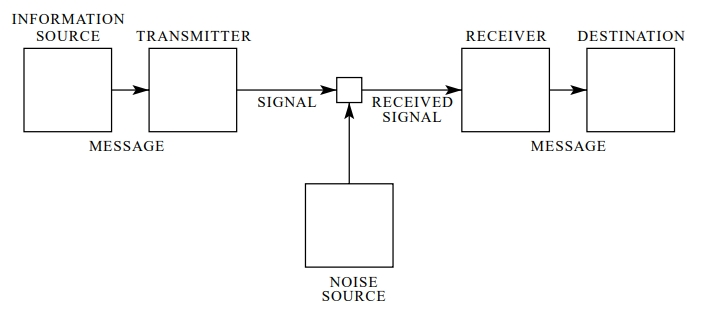
\includegraphics[width=0.6\textwidth]{assets/engineering_communication_system.jpg}
			\caption{Schematic diagram of an engineering/technical communication system \cite{Shannon1948}}
		\end{figure}
		\begin{exampleblock}{A Mathematical Theory of Communication \cite{Shannon1948}\hspace*\fill--- C. E. Shannon}
			The fundamental problem of communication is that of reproducing at one point either exactly or approximately a message selected at another point. Frequently the messages have \alert{\emph{meaning;}} that is they refer to or are correlated according to some system with certain physical or conceptual entities. \alert{These semantic aspects of communication are irrelevant to the engineering problem.}
			% \hspace*\fill{\small--- C. E. Shannon}
		\end{exampleblock}
		\singlespacing
		Did Shannon intentionally excluded semantics from information theory?
	\end{frame}

	\begin{frame}{Three Levels of Communications}
		\begin{figure}
			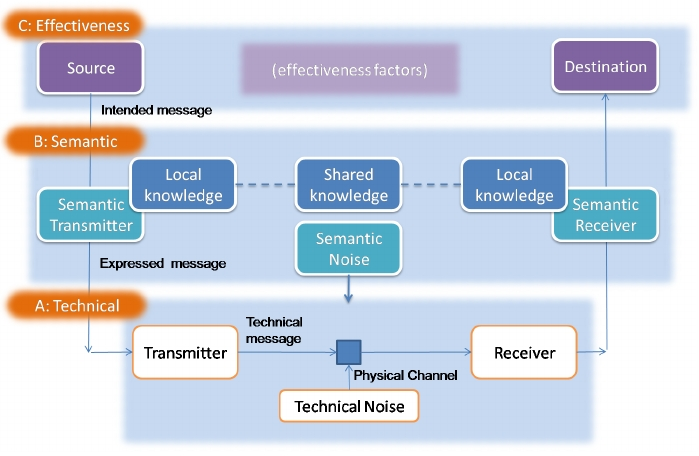
\includegraphics[width=0.6\textwidth]{assets/3_level_communication_model.jpg}
			\caption{A 3-level communication model \cite{Bao2011}}
		\end{figure}
		\vspace{-0.4cm}
		% \begin{exampleblock}{Recent Contributions to the Mathematical Theory of Communication \cite{Weaver1953}\\\hspace*\fill--- W. Weaver}
		\begin{exampleblock}{Three Levels of Communications \cite{Weaver1953}\hspace*\fill--- W. Weaver}
			\begin{itemize}
				\item Level A. How accurately can the symbols of communication be transmitted? (The \alert{technical} problem.)
				\item Level B. How precisely do the transmitted symbols convey the desired meaning? (The \alert{semantic} problem.)
				\item Level C. How effectively does the received meaning affect conduct in the desired way? (The \alert{effectiveness} problem.)
			\end{itemize}
			% \hspace*\fill{\small--- W. Weaver}
		\end{exampleblock}
	\end{frame}
\end{section}



\bibliographystyle{IEEEtran}
\bibliography{IEEEabrv,library.bib}
\end{document}
